\documentclass[1p]{elsarticle_modified}
%\bibliographystyle{elsarticle-num}

%\usepackage[colorlinks]{hyperref}
%\usepackage{abbrmath_seonhwa} %\Abb, \Ascr, \Acal ,\Abf, \Afrak
\usepackage{amsfonts}
\usepackage{amssymb}
\usepackage{amsmath}
\usepackage{amsthm}
\usepackage{scalefnt}
\usepackage{amsbsy}
\usepackage{kotex}
\usepackage{caption}
\usepackage{subfig}
\usepackage{color}
\usepackage{graphicx}
\usepackage{xcolor} %% white, black, red, green, blue, cyan, magenta, yellow
\usepackage{float}
\usepackage{setspace}
\usepackage{hyperref}

\usepackage{tikz}
\usetikzlibrary{arrows}

\usepackage{multirow}
\usepackage{array} % fixed length table
\usepackage{hhline}

%%%%%%%%%%%%%%%%%%%%%
\makeatletter
\renewcommand*\env@matrix[1][\arraystretch]{%
	\edef\arraystretch{#1}%
	\hskip -\arraycolsep
	\let\@ifnextchar\new@ifnextchar
	\array{*\c@MaxMatrixCols c}}
\makeatother %https://tex.stackexchange.com/questions/14071/how-can-i-increase-the-line-spacing-in-a-matrix
%%%%%%%%%%%%%%%

\usepackage[normalem]{ulem}

\newcommand{\msout}[1]{\ifmmode\text{\sout{\ensuremath{#1}}}\else\sout{#1}\fi}
%SOURCE: \msout is \stkout macro in https://tex.stackexchange.com/questions/20609/strikeout-in-math-mode

\newcommand{\cancel}[1]{
	\ifmmode
	{\color{red}\msout{#1}}
	\else
	{\color{red}\sout{#1}}
	\fi
}

\newcommand{\add}[1]{
	{\color{blue}\uwave{#1}}
}

\newcommand{\replace}[2]{
	\ifmmode
	{\color{red}\msout{#1}}{\color{blue}\uwave{#2}}
	\else
	{\color{red}\sout{#1}}{\color{blue}\uwave{#2}}
	\fi
}

\newcommand{\Sol}{\mathcal{S}} %segment
\newcommand{\D}{D} %diagram
\newcommand{\A}{\mathcal{A}} %arc


%%%%%%%%%%%%%%%%%%%%%%%%%%%%%5 test

\def\sl{\operatorname{\textup{SL}}(2,\Cbb)}
\def\psl{\operatorname{\textup{PSL}}(2,\Cbb)}
\def\quan{\mkern 1mu \triangleright \mkern 1mu}

\theoremstyle{definition}
\newtheorem{thm}{Theorem}[section]
\newtheorem{prop}[thm]{Proposition}
\newtheorem{lem}[thm]{Lemma}
\newtheorem{ques}[thm]{Question}
\newtheorem{cor}[thm]{Corollary}
\newtheorem{defn}[thm]{Definition}
\newtheorem{exam}[thm]{Example}
\newtheorem{rmk}[thm]{Remark}
\newtheorem{alg}[thm]{Algorithm}

\newcommand{\I}{\sqrt{-1}}
\begin{document}

%\begin{frontmatter}
%
%\title{Boundary parabolic representations of knots up to 8 crossings}
%
%%% Group authors per affiliation:
%\author{Yunhi Cho} 
%\address{Department of Mathematics, University of Seoul, Seoul, Korea}
%\ead{yhcho@uos.ac.kr}
%
%
%\author{Seonhwa Kim} %\fnref{s_kim}}
%\address{Center for Geometry and Physics, Institute for Basic Science, Pohang, 37673, Korea}
%\ead{ryeona17@ibs.re.kr}
%
%\author{Hyuk Kim}
%\address{Department of Mathematical Sciences, Seoul National University, Seoul 08826, Korea}
%\ead{hyukkim@snu.ac.kr}
%
%\author{Seokbeom Yoon}
%\address{Department of Mathematical Sciences, Seoul National University, Seoul, 08826,  Korea}
%\ead{sbyoon15@snu.ac.kr}
%
%\begin{abstract}
%We find all boundary parabolic representation of knots up to 8 crossings.
%
%\end{abstract}
%\begin{keyword}
%    \MSC[2010] 57M25 
%\end{keyword}
%
%\end{frontmatter}

%\linenumbers
%\tableofcontents
%
\newcommand\colored[1]{\textcolor{white}{\rule[-0.35ex]{0.8em}{1.4ex}}\kern-0.8em\color{red} #1}%
%\newcommand\colored[1]{\textcolor{white}{ #1}\kern-2.17ex	\textcolor{white}{ #1}\kern-1.81ex	\textcolor{white}{ #1}\kern-2.15ex\color{red}#1	}

{\Large $\underline{12a_{1075}~(K12a_{1075})}$}

\setlength{\tabcolsep}{10pt}
\renewcommand{\arraystretch}{1.6}
\vspace{1cm}\begin{tabular}{m{100pt}>{\centering\arraybackslash}m{274pt}}
\multirow{5}{120pt}{
	\centering
	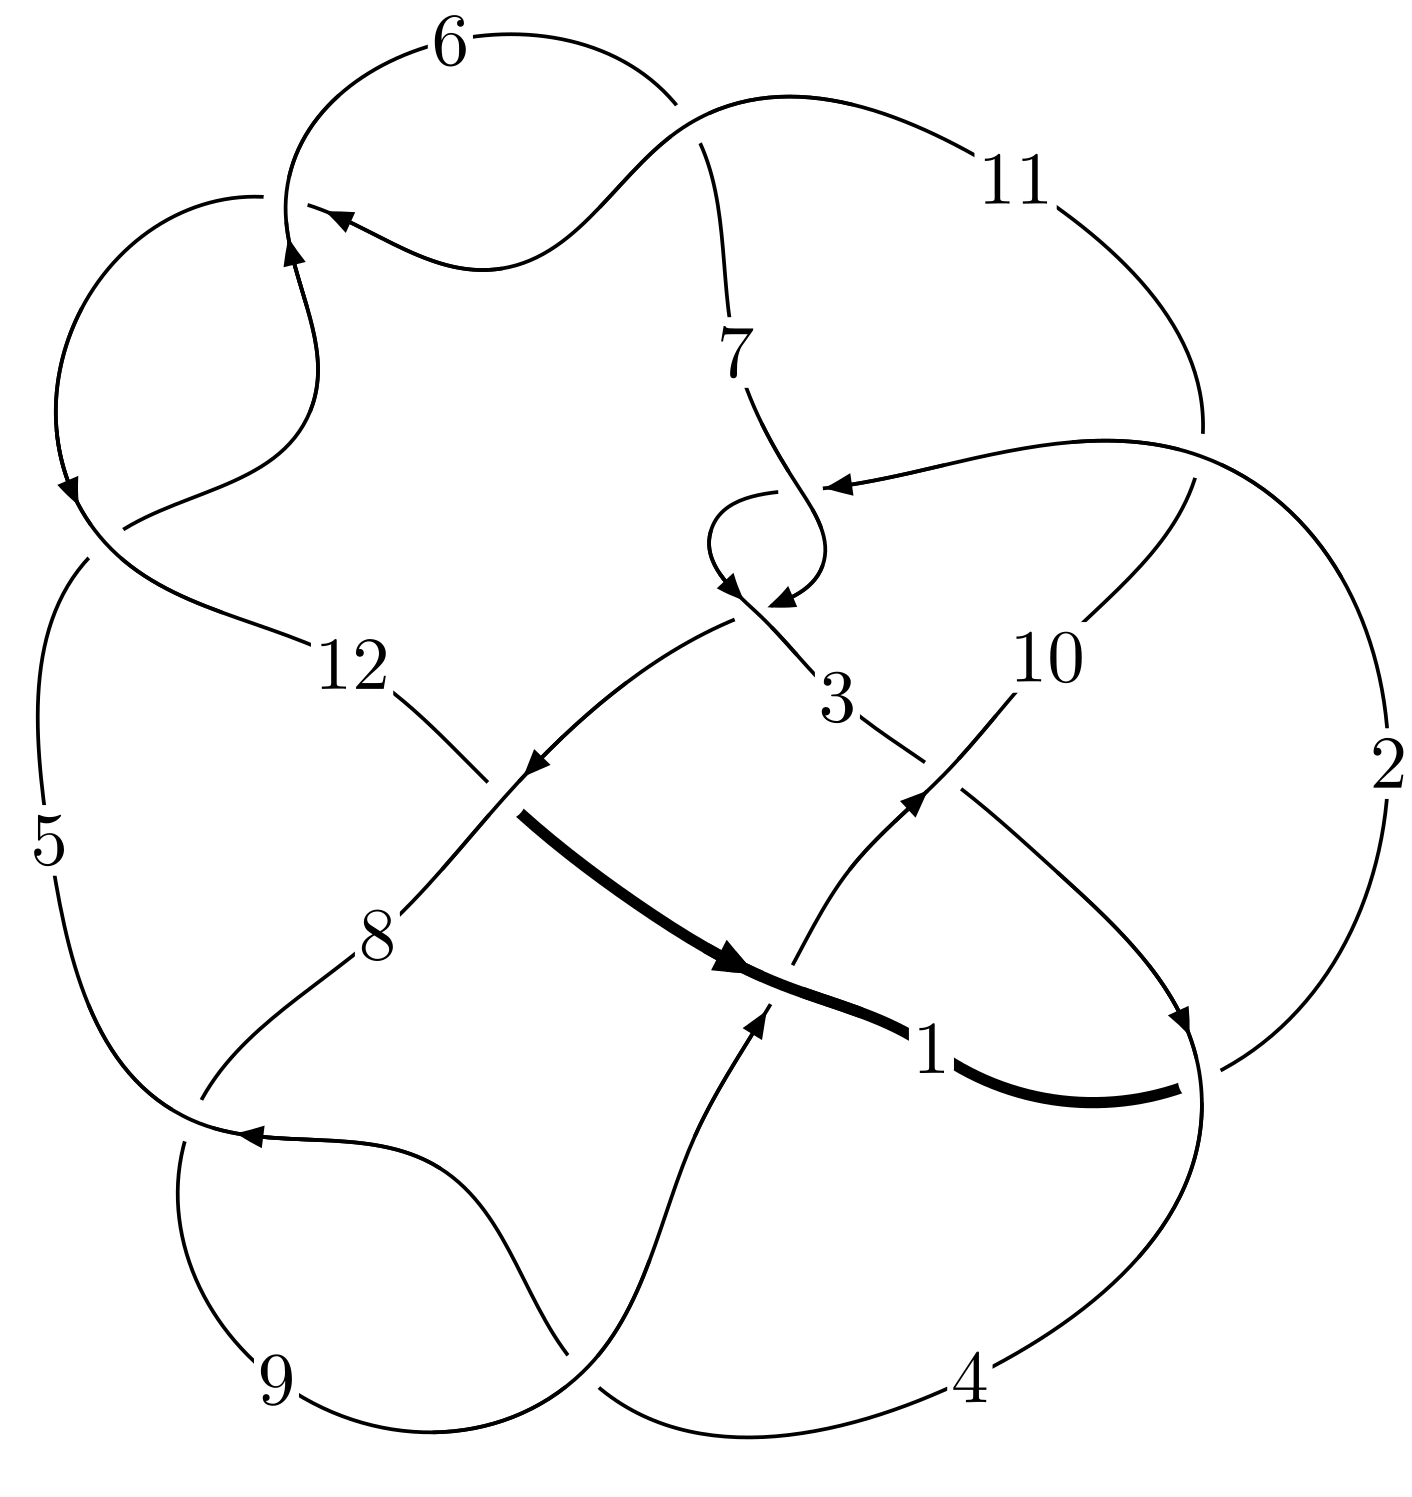
\includegraphics[width=112pt]{../../../GIT/diagram.site/Diagrams/png/1876_12a_1075.png}\\
\ \ \ A knot diagram\footnotemark}&
\allowdisplaybreaks
\textbf{Linearized knot diagam} \\
\cline{2-2}
 &
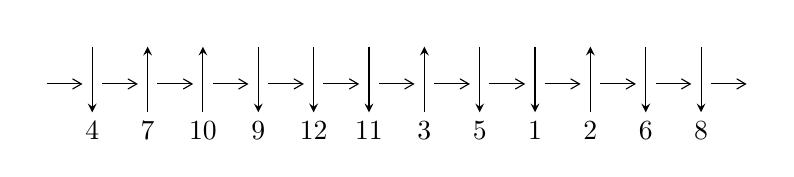
\begin{tikzpicture}[x=20pt, y=17pt]
	% nodes
	\node (C0) at (0, 0) {};
	\node (C1) at (1, 0) {};
	\node (C1U) at (1, +1) {};
	\node (C1D) at (1, -1) {4};

	\node (C2) at (2, 0) {};
	\node (C2U) at (2, +1) {};
	\node (C2D) at (2, -1) {7};

	\node (C3) at (3, 0) {};
	\node (C3U) at (3, +1) {};
	\node (C3D) at (3, -1) {10};

	\node (C4) at (4, 0) {};
	\node (C4U) at (4, +1) {};
	\node (C4D) at (4, -1) {9};

	\node (C5) at (5, 0) {};
	\node (C5U) at (5, +1) {};
	\node (C5D) at (5, -1) {12};

	\node (C6) at (6, 0) {};
	\node (C6U) at (6, +1) {};
	\node (C6D) at (6, -1) {11};

	\node (C7) at (7, 0) {};
	\node (C7U) at (7, +1) {};
	\node (C7D) at (7, -1) {3};

	\node (C8) at (8, 0) {};
	\node (C8U) at (8, +1) {};
	\node (C8D) at (8, -1) {5};

	\node (C9) at (9, 0) {};
	\node (C9U) at (9, +1) {};
	\node (C9D) at (9, -1) {1};

	\node (C10) at (10, 0) {};
	\node (C10U) at (10, +1) {};
	\node (C10D) at (10, -1) {2};

	\node (C11) at (11, 0) {};
	\node (C11U) at (11, +1) {};
	\node (C11D) at (11, -1) {6};

	\node (C12) at (12, 0) {};
	\node (C12U) at (12, +1) {};
	\node (C12D) at (12, -1) {8};
	\node (C13) at (13, 0) {};

	% arrows
	\draw[->,>={angle 60}]
	(C0) edge (C1) (C1) edge (C2) (C2) edge (C3) (C3) edge (C4) (C4) edge (C5) (C5) edge (C6) (C6) edge (C7) (C7) edge (C8) (C8) edge (C9) (C9) edge (C10) (C10) edge (C11) (C11) edge (C12) (C12) edge (C13) ;	\draw[->,>=stealth]
	(C1U) edge (C1D) (C2D) edge (C2U) (C3D) edge (C3U) (C4U) edge (C4D) (C5U) edge (C5D) (C6U) edge (C6D) (C7D) edge (C7U) (C8U) edge (C8D) (C9U) edge (C9D) (C10D) edge (C10U) (C11U) edge (C11D) (C12U) edge (C12D) ;
	\end{tikzpicture} \\
\hhline{~~} \\& 
\textbf{Solving Sequence} \\ \cline{2-2} 
 &
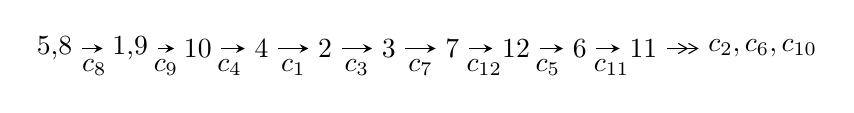
\begin{tikzpicture}[x=23pt, y=7pt]
	% node
	\node (A0) at (-1/8, 0) {5,8};
	\node (A1) at (17/16, 0) {1,9};
	\node (A2) at (17/8, 0) {10};
	\node (A3) at (25/8, 0) {4};
	\node (A4) at (33/8, 0) {2};
	\node (A5) at (41/8, 0) {3};
	\node (A6) at (49/8, 0) {7};
	\node (A7) at (57/8, 0) {12};
	\node (A8) at (65/8, 0) {6};
	\node (A9) at (73/8, 0) {11};
	\node (C1) at (1/2, -1) {$c_{8}$};
	\node (C2) at (13/8, -1) {$c_{9}$};
	\node (C3) at (21/8, -1) {$c_{4}$};
	\node (C4) at (29/8, -1) {$c_{1}$};
	\node (C5) at (37/8, -1) {$c_{3}$};
	\node (C6) at (45/8, -1) {$c_{7}$};
	\node (C7) at (53/8, -1) {$c_{12}$};
	\node (C8) at (61/8, -1) {$c_{5}$};
	\node (C9) at (69/8, -1) {$c_{11}$};
	\node (A10) at (11, 0) {$c_{2},c_{6},c_{10}$};

	% edge
	\draw[->,>=stealth]	
	(A0) edge (A1) (A1) edge (A2) (A2) edge (A3) (A3) edge (A4) (A4) edge (A5) (A5) edge (A6) (A6) edge (A7) (A7) edge (A8) (A8) edge (A9) ;
	\draw[->>,>={angle 60}]	
	(A9) edge (A10);
\end{tikzpicture} \\ 

\end{tabular} \\

\footnotetext{
The image of knot diagram is generated by the software ``\textbf{Draw programme}" developed by Andrew Bartholomew(\url{http://www.layer8.co.uk/maths/draw/index.htm\#Running-draw}), where we modified some parts for our purpose(\url{https://github.com/CATsTAILs/LinksPainter}).
}\phantom \\ \newline 
\centering \textbf{Ideals for irreducible components\footnotemark of $X_{\text{par}}$} 
 
\begin{align*}
I^u_{1}&=\langle 
3.72612\times10^{441} u^{119}+2.23519\times10^{442} u^{118}+\cdots+6.93517\times10^{441} b+7.61910\times10^{442},\\
\phantom{I^u_{1}}&\phantom{= \langle  }-1.13200\times10^{442} u^{119}-8.72311\times10^{442} u^{118}+\cdots+2.77407\times10^{442} a-2.01129\times10^{443},\\
\phantom{I^u_{1}}&\phantom{= \langle  }u^{120}+4 u^{119}+\cdots+176 u+16\rangle \\
I^u_{2}&=\langle 
-11729899 u^{29}+392758785 u^{28}+\cdots+663256056 b-336061032,\\
\phantom{I^u_{2}}&\phantom{= \langle  }313877822 u^{29}-659380977 u^{28}+\cdots+663256056 a+3199377682,\;u^{30}- u^{29}+\cdots+16 u+4\rangle \\
\\
\end{align*}
\raggedright * 2 irreducible components of $\dim_{\mathbb{C}}=0$, with total 150 representations.\\
\footnotetext{All coefficients of polynomials are rational numbers. But the coefficients are sometimes approximated in decimal forms when there is not enough margin.}
\newpage
\renewcommand{\arraystretch}{1}
\centering \section*{I. $I^u_{1}= \langle 3.73\times10^{441} u^{119}+2.24\times10^{442} u^{118}+\cdots+6.94\times10^{441} b+7.62\times10^{442},\;-1.13\times10^{442} u^{119}-8.72\times10^{442} u^{118}+\cdots+2.77\times10^{442} a-2.01\times10^{443},\;u^{120}+4 u^{119}+\cdots+176 u+16 \rangle$}
\flushleft \textbf{(i) Arc colorings}\\
\begin{tabular}{m{7pt} m{180pt} m{7pt} m{180pt} }
\flushright $a_{5}=$&$\begin{pmatrix}0\\u\end{pmatrix}$ \\
\flushright $a_{8}=$&$\begin{pmatrix}1\\0\end{pmatrix}$ \\
\flushright $a_{1}=$&$\begin{pmatrix}0.408064 u^{119}+3.14452 u^{118}+\cdots+149.127 u+7.25033\\-0.537279 u^{119}-3.22299 u^{118}+\cdots-126.152 u-10.9862\end{pmatrix}$ \\
\flushright $a_{9}=$&$\begin{pmatrix}1\\u^2\end{pmatrix}$ \\
\flushright $a_{10}=$&$\begin{pmatrix}0.133061 u^{119}-1.76548 u^{118}+\cdots-287.316 u-19.5313\\0.157698 u^{119}+0.894253 u^{118}+\cdots+28.6860 u+1.72084\end{pmatrix}$ \\
\flushright $a_{4}=$&$\begin{pmatrix}u\\u^3+u\end{pmatrix}$ \\
\flushright $a_{2}=$&$\begin{pmatrix}0.0309732 u^{119}+1.11273 u^{118}+\cdots+80.2324 u+1.22501\\-0.286921 u^{119}-2.01484 u^{118}+\cdots-96.8888 u-8.63661\end{pmatrix}$ \\
\flushright $a_{3}=$&$\begin{pmatrix}-1.30794 u^{119}-5.76141 u^{118}+\cdots-133.536 u-9.65675\\-0.320020 u^{119}-1.44002 u^{118}+\cdots-32.1909 u-3.68571\end{pmatrix}$ \\
\flushright $a_{7}=$&$\begin{pmatrix}-1.21287 u^{119}-5.16416 u^{118}+\cdots+49.6915 u+7.33530\\0.143813 u^{119}+0.399070 u^{118}+\cdots-25.2449 u-1.30807\end{pmatrix}$ \\
\flushright $a_{12}=$&$\begin{pmatrix}-0.129215 u^{119}-0.0784645 u^{118}+\cdots+22.9748 u-3.73586\\-0.537279 u^{119}-3.22299 u^{118}+\cdots-126.152 u-10.9862\end{pmatrix}$ \\
\flushright $a_{6}=$&$\begin{pmatrix}0.976745 u^{119}+4.50726 u^{118}+\cdots+53.6799 u+5.26035\\-1.14558 u^{119}-3.97966 u^{118}+\cdots+37.4447 u+4.69013\end{pmatrix}$ \\
\flushright $a_{11}=$&$\begin{pmatrix}0.841118 u^{119}+1.64638 u^{118}+\cdots-264.638 u-25.8472\\0.0713272 u^{119}+1.27908 u^{118}+\cdots+113.008 u+10.1802\end{pmatrix}$\\&\end{tabular}
\flushleft \textbf{(ii) Obstruction class $= -1$}\\~\\
\flushleft \textbf{(iii) Cusp Shapes $= 2.82220 u^{119}+11.1817 u^{118}+\cdots+52.9511 u+4.35858$}\\~\\
\newpage\renewcommand{\arraystretch}{1}
\flushleft \textbf{(iv) u-Polynomials at the component}\newline \\
\begin{tabular}{m{50pt}|m{274pt}}
Crossings & \hspace{64pt}u-Polynomials at each crossing \\
\hline $$\begin{aligned}c_{1}\end{aligned}$$&$\begin{aligned}
&u^{120}-12 u^{119}+\cdots-105451 u+8381
\end{aligned}$\\
\hline $$\begin{aligned}c_{2},c_{7}\end{aligned}$$&$\begin{aligned}
&u^{120}+2 u^{119}+\cdots-10425 u+6379
\end{aligned}$\\
\hline $$\begin{aligned}c_{3}\end{aligned}$$&$\begin{aligned}
&u^{120}+u^{119}+\cdots+172 u+11
\end{aligned}$\\
\hline $$\begin{aligned}c_{4},c_{8}\end{aligned}$$&$\begin{aligned}
&u^{120}+4 u^{119}+\cdots+176 u+16
\end{aligned}$\\
\hline $$\begin{aligned}c_{5},c_{6},c_{11}\end{aligned}$$&$\begin{aligned}
&u^{120}- u^{119}+\cdots-4711 u+667
\end{aligned}$\\
\hline $$\begin{aligned}c_{9}\end{aligned}$$&$\begin{aligned}
&u^{120}-4 u^{119}+\cdots+42 u+11
\end{aligned}$\\
\hline $$\begin{aligned}c_{10}\end{aligned}$$&$\begin{aligned}
&u^{120}-30 u^{118}+\cdots-6834664 u+20792117
\end{aligned}$\\
\hline $$\begin{aligned}c_{12}\end{aligned}$$&$\begin{aligned}
&u^{120}+u^{119}+\cdots+84308126 u+35235131
\end{aligned}$\\
\hline
\end{tabular}\\~\\
\newpage\renewcommand{\arraystretch}{1}
\flushleft \textbf{(v) Riley Polynomials at the component}\newline \\
\begin{tabular}{m{50pt}|m{274pt}}
Crossings & \hspace{64pt}Riley Polynomials at each crossing \\
\hline $$\begin{aligned}c_{1}\end{aligned}$$&$\begin{aligned}
&y^{120}+36 y^{119}+\cdots+4420639659 y+70241161
\end{aligned}$\\
\hline $$\begin{aligned}c_{2},c_{7}\end{aligned}$$&$\begin{aligned}
&y^{120}-84 y^{119}+\cdots-765539013 y+40691641
\end{aligned}$\\
\hline $$\begin{aligned}c_{3}\end{aligned}$$&$\begin{aligned}
&y^{120}+15 y^{119}+\cdots+5726 y+121
\end{aligned}$\\
\hline $$\begin{aligned}c_{4},c_{8}\end{aligned}$$&$\begin{aligned}
&y^{120}+102 y^{119}+\cdots-6912 y+256
\end{aligned}$\\
\hline $$\begin{aligned}c_{5},c_{6},c_{11}\end{aligned}$$&$\begin{aligned}
&y^{120}+141 y^{119}+\cdots+27200497 y+444889
\end{aligned}$\\
\hline $$\begin{aligned}c_{9}\end{aligned}$$&$\begin{aligned}
&y^{120}+110 y^{118}+\cdots+5298 y+121
\end{aligned}$\\
\hline $$\begin{aligned}c_{10}\end{aligned}$$&$\begin{aligned}
&y^{120}-60 y^{119}+\cdots-3535423773129192 y+432312129341689
\end{aligned}$\\
\hline $$\begin{aligned}c_{12}\end{aligned}$$&$\begin{aligned}
&y^{120}+67 y^{119}+\cdots+44858396743231608 y+1241514456587161
\end{aligned}$\\
\hline
\end{tabular}\\~\\
\newpage\flushleft \textbf{(vi) Complex Volumes and Cusp Shapes}
$$\begin{array}{c|c|c}  
\text{Solutions to }I^u_{1}& \I (\text{vol} + \sqrt{-1}CS) & \text{Cusp shape}\\
 \hline 
\begin{aligned}
u &= \phantom{-}0.997060 + 0.155292 I \\
a &= \phantom{-}0.0384016 + 0.1145680 I \\
b &= -0.842177 - 0.631123 I\end{aligned}
 & \phantom{-}1.98018 - 8.81242 I & \phantom{-0.000000 } 0 \\ \hline\begin{aligned}
u &= \phantom{-}0.997060 - 0.155292 I \\
a &= \phantom{-}0.0384016 - 0.1145680 I \\
b &= -0.842177 + 0.631123 I\end{aligned}
 & \phantom{-}1.98018 + 8.81242 I & \phantom{-0.000000 } 0 \\ \hline\begin{aligned}
u &= -0.601243 + 0.771166 I \\
a &= \phantom{-}0.813940 + 0.283363 I \\
b &= -0.621526 - 0.557357 I\end{aligned}
 & -0.92514 + 2.55810 I & \phantom{-0.000000 } 0 \\ \hline\begin{aligned}
u &= -0.601243 - 0.771166 I \\
a &= \phantom{-}0.813940 - 0.283363 I \\
b &= -0.621526 + 0.557357 I\end{aligned}
 & -0.92514 - 2.55810 I & \phantom{-0.000000 } 0 \\ \hline\begin{aligned}
u &= -1.037890 + 0.181103 I \\
a &= \phantom{-}0.180007 - 0.080743 I \\
b &= -0.571054 + 0.389492 I\end{aligned}
 & -1.76846 + 3.67590 I & \phantom{-0.000000 } 0 \\ \hline\begin{aligned}
u &= -1.037890 - 0.181103 I \\
a &= \phantom{-}0.180007 + 0.080743 I \\
b &= -0.571054 - 0.389492 I\end{aligned}
 & -1.76846 - 3.67590 I & \phantom{-0.000000 } 0 \\ \hline\begin{aligned}
u &= \phantom{-}0.647251 + 0.834053 I \\
a &= -1.30505 + 0.63619 I \\
b &= \phantom{-}0.15586 - 1.50651 I\end{aligned}
 & \phantom{-}5.36355 - 2.53103 I & \phantom{-0.000000 } 0 \\ \hline\begin{aligned}
u &= \phantom{-}0.647251 - 0.834053 I \\
a &= -1.30505 - 0.63619 I \\
b &= \phantom{-}0.15586 + 1.50651 I\end{aligned}
 & \phantom{-}5.36355 + 2.53103 I & \phantom{-0.000000 } 0 \\ \hline\begin{aligned}
u &= -0.264406 + 0.899217 I \\
a &= \phantom{-}0.274431 + 1.247060 I \\
b &= \phantom{-}0.241776 - 0.902567 I\end{aligned}
 & -0.43312 + 1.50393 I & \phantom{-0.000000 } 0 \\ \hline\begin{aligned}
u &= -0.264406 - 0.899217 I \\
a &= \phantom{-}0.274431 - 1.247060 I \\
b &= \phantom{-}0.241776 + 0.902567 I\end{aligned}
 & -0.43312 - 1.50393 I & \phantom{-0.000000 } 0\\
 \hline 
 \end{array}$$\newpage$$\begin{array}{c|c|c}  
\text{Solutions to }I^u_{1}& \I (\text{vol} + \sqrt{-1}CS) & \text{Cusp shape}\\
 \hline 
\begin{aligned}
u &= -0.080116 + 1.065280 I \\
a &= \phantom{-}0.71043 - 1.30579 I \\
b &= -0.578713 + 0.719695 I\end{aligned}
 & \phantom{-}2.15815 + 2.38721 I & \phantom{-0.000000 } 0 \\ \hline\begin{aligned}
u &= -0.080116 - 1.065280 I \\
a &= \phantom{-}0.71043 + 1.30579 I \\
b &= -0.578713 - 0.719695 I\end{aligned}
 & \phantom{-}2.15815 - 2.38721 I & \phantom{-0.000000 } 0 \\ \hline\begin{aligned}
u &= \phantom{-}0.163464 + 0.913347 I \\
a &= -0.577288 + 0.465106 I \\
b &= \phantom{-}1.41344 - 0.24530 I\end{aligned}
 & \phantom{-}0.43101 - 2.97537 I & \phantom{-0.000000 } 0 \\ \hline\begin{aligned}
u &= \phantom{-}0.163464 - 0.913347 I \\
a &= -0.577288 - 0.465106 I \\
b &= \phantom{-}1.41344 + 0.24530 I\end{aligned}
 & \phantom{-}0.43101 + 2.97537 I & \phantom{-0.000000 } 0 \\ \hline\begin{aligned}
u &= \phantom{-}0.259984 + 1.099700 I \\
a &= -0.30600 - 1.79640 I \\
b &= \phantom{-}1.01869 + 1.51224 I\end{aligned}
 & \phantom{-}3.73125 - 6.13320 I & \phantom{-0.000000 } 0 \\ \hline\begin{aligned}
u &= \phantom{-}0.259984 - 1.099700 I \\
a &= -0.30600 + 1.79640 I \\
b &= \phantom{-}1.01869 - 1.51224 I\end{aligned}
 & \phantom{-}3.73125 + 6.13320 I & \phantom{-0.000000 } 0 \\ \hline\begin{aligned}
u &= \phantom{-}0.792528 + 0.326858 I \\
a &= -0.111014 - 0.451742 I \\
b &= -0.618881 - 0.852939 I\end{aligned}
 & \phantom{-}2.71259 - 2.58388 I & \phantom{-0.000000 } 0 \\ \hline\begin{aligned}
u &= \phantom{-}0.792528 - 0.326858 I \\
a &= -0.111014 + 0.451742 I \\
b &= -0.618881 + 0.852939 I\end{aligned}
 & \phantom{-}2.71259 + 2.58388 I & \phantom{-0.000000 } 0 \\ \hline\begin{aligned}
u &= \phantom{-}0.854709 + 0.000169 I \\
a &= \phantom{-}0.432488 + 0.076734 I \\
b &= \phantom{-}0.162238 - 0.730395 I\end{aligned}
 & \phantom{-}3.97435 - 0.08833 I & \phantom{-0.000000 } 0 \\ \hline\begin{aligned}
u &= \phantom{-}0.854709 - 0.000169 I \\
a &= \phantom{-}0.432488 - 0.076734 I \\
b &= \phantom{-}0.162238 + 0.730395 I\end{aligned}
 & \phantom{-}3.97435 + 0.08833 I & \phantom{-0.000000 } 0\\
 \hline 
 \end{array}$$\newpage$$\begin{array}{c|c|c}  
\text{Solutions to }I^u_{1}& \I (\text{vol} + \sqrt{-1}CS) & \text{Cusp shape}\\
 \hline 
\begin{aligned}
u &= -0.795264 + 0.153084 I \\
a &= \phantom{-}0.287557 + 0.595180 I \\
b &= -0.658467 + 1.205740 I\end{aligned}
 & \phantom{-}4.86393 + 3.48843 I & \phantom{-0.000000 } 0 \\ \hline\begin{aligned}
u &= -0.795264 - 0.153084 I \\
a &= \phantom{-}0.287557 - 0.595180 I \\
b &= -0.658467 - 1.205740 I\end{aligned}
 & \phantom{-}4.86393 - 3.48843 I & \phantom{-0.000000 } 0 \\ \hline\begin{aligned}
u &= -0.328756 + 1.146120 I \\
a &= -0.08218 - 2.18274 I \\
b &= -1.24715 + 2.43802 I\end{aligned}
 & \phantom{-}11.5929 + 8.5289 I & \phantom{-0.000000 } 0 \\ \hline\begin{aligned}
u &= -0.328756 - 1.146120 I \\
a &= -0.08218 + 2.18274 I \\
b &= -1.24715 - 2.43802 I\end{aligned}
 & \phantom{-}11.5929 - 8.5289 I & \phantom{-0.000000 } 0 \\ \hline\begin{aligned}
u &= -0.113420 + 1.208560 I \\
a &= -0.66599 - 1.88489 I \\
b &= \phantom{-}1.02115 + 1.93305 I\end{aligned}
 & \phantom{-}7.02433 + 5.04561 I & \phantom{-0.000000 } 0 \\ \hline\begin{aligned}
u &= -0.113420 - 1.208560 I \\
a &= -0.66599 + 1.88489 I \\
b &= \phantom{-}1.02115 - 1.93305 I\end{aligned}
 & \phantom{-}7.02433 - 5.04561 I & \phantom{-0.000000 } 0 \\ \hline\begin{aligned}
u &= -0.716768 + 0.293774 I \\
a &= -1.27622 + 0.85814 I \\
b &= \phantom{-}0.607399 + 1.103350 I\end{aligned}
 & \phantom{-}9.05152 - 4.61063 I & \phantom{-0.000000 } 0 \\ \hline\begin{aligned}
u &= -0.716768 - 0.293774 I \\
a &= -1.27622 - 0.85814 I \\
b &= \phantom{-}0.607399 - 1.103350 I\end{aligned}
 & \phantom{-}9.05152 + 4.61063 I & \phantom{-0.000000 } 0 \\ \hline\begin{aligned}
u &= \phantom{-}0.005789 + 1.229110 I \\
a &= -1.133040 - 0.812110 I \\
b &= -0.556977 + 0.460644 I\end{aligned}
 & \phantom{-}11.88010 + 1.14020 I & \phantom{-0.000000 } 0 \\ \hline\begin{aligned}
u &= \phantom{-}0.005789 - 1.229110 I \\
a &= -1.133040 + 0.812110 I \\
b &= -0.556977 - 0.460644 I\end{aligned}
 & \phantom{-}11.88010 - 1.14020 I & \phantom{-0.000000 } 0\\
 \hline 
 \end{array}$$\newpage$$\begin{array}{c|c|c}  
\text{Solutions to }I^u_{1}& \I (\text{vol} + \sqrt{-1}CS) & \text{Cusp shape}\\
 \hline 
\begin{aligned}
u &= -0.458346 + 1.143630 I \\
a &= -0.958222 - 0.481606 I \\
b &= -0.276910 + 0.789615 I\end{aligned}
 & \phantom{-}7.74673 + 0.95719 I & \phantom{-0.000000 } 0 \\ \hline\begin{aligned}
u &= -0.458346 - 1.143630 I \\
a &= -0.958222 + 0.481606 I \\
b &= -0.276910 - 0.789615 I\end{aligned}
 & \phantom{-}7.74673 - 0.95719 I & \phantom{-0.000000 } 0 \\ \hline\begin{aligned}
u &= \phantom{-}0.068494 + 1.231050 I \\
a &= -0.156613 - 1.337530 I \\
b &= -0.306630 + 0.831609 I\end{aligned}
 & \phantom{-}3.88824 + 0.70963 I & \phantom{-0.000000 } 0 \\ \hline\begin{aligned}
u &= \phantom{-}0.068494 - 1.231050 I \\
a &= -0.156613 + 1.337530 I \\
b &= -0.306630 - 0.831609 I\end{aligned}
 & \phantom{-}3.88824 - 0.70963 I & \phantom{-0.000000 } 0 \\ \hline\begin{aligned}
u &= \phantom{-}0.023307 + 1.236670 I \\
a &= \phantom{-}0.198656 + 1.334160 I \\
b &= -1.49023 - 1.25302 I\end{aligned}
 & \phantom{-}9.11727 + 1.44245 I & \phantom{-0.000000 } 0 \\ \hline\begin{aligned}
u &= \phantom{-}0.023307 - 1.236670 I \\
a &= \phantom{-}0.198656 - 1.334160 I \\
b &= -1.49023 + 1.25302 I\end{aligned}
 & \phantom{-}9.11727 - 1.44245 I & \phantom{-0.000000 } 0 \\ \hline\begin{aligned}
u &= -0.043678 + 1.236630 I \\
a &= -0.33976 + 1.91669 I \\
b &= -0.251642 - 1.008870 I\end{aligned}
 & \phantom{-}7.43407 - 3.48374 I & \phantom{-0.000000 } 0 \\ \hline\begin{aligned}
u &= -0.043678 - 1.236630 I \\
a &= -0.33976 - 1.91669 I \\
b &= -0.251642 + 1.008870 I\end{aligned}
 & \phantom{-}7.43407 + 3.48374 I & \phantom{-0.000000 } 0 \\ \hline\begin{aligned}
u &= \phantom{-}0.172706 + 1.228910 I \\
a &= -0.924628 - 0.655584 I \\
b &= \phantom{-}0.181142 + 0.194501 I\end{aligned}
 & \phantom{-}5.04503 + 0.67908 I & \phantom{-0.000000 } 0 \\ \hline\begin{aligned}
u &= \phantom{-}0.172706 - 1.228910 I \\
a &= -0.924628 + 0.655584 I \\
b &= \phantom{-}0.181142 - 0.194501 I\end{aligned}
 & \phantom{-}5.04503 - 0.67908 I & \phantom{-0.000000 } 0\\
 \hline 
 \end{array}$$\newpage$$\begin{array}{c|c|c}  
\text{Solutions to }I^u_{1}& \I (\text{vol} + \sqrt{-1}CS) & \text{Cusp shape}\\
 \hline 
\begin{aligned}
u &= -0.073238 + 1.240730 I \\
a &= \phantom{-}0.68583 - 2.22932 I \\
b &= -1.92385 + 2.33511 I\end{aligned}
 & \phantom{-}13.8536 - 5.5955 I & \phantom{-0.000000 } 0 \\ \hline\begin{aligned}
u &= -0.073238 - 1.240730 I \\
a &= \phantom{-}0.68583 + 2.22932 I \\
b &= -1.92385 - 2.33511 I\end{aligned}
 & \phantom{-}13.8536 + 5.5955 I & \phantom{-0.000000 } 0 \\ \hline\begin{aligned}
u &= \phantom{-}0.260529 + 1.215970 I \\
a &= \phantom{-}0.13896 + 1.51889 I \\
b &= \phantom{-}0.032878 - 0.913255 I\end{aligned}
 & \phantom{-}2.03580 - 4.58641 I & \phantom{-0.000000 } 0 \\ \hline\begin{aligned}
u &= \phantom{-}0.260529 - 1.215970 I \\
a &= \phantom{-}0.13896 - 1.51889 I \\
b &= \phantom{-}0.032878 + 0.913255 I\end{aligned}
 & \phantom{-}2.03580 + 4.58641 I & \phantom{-0.000000 } 0 \\ \hline\begin{aligned}
u &= -1.200470 + 0.341560 I \\
a &= -0.080500 - 0.196637 I \\
b &= \phantom{-}0.597030 - 0.974530 I\end{aligned}
 & \phantom{-}9.3530 + 12.2656 I & \phantom{-0.000000 } 0 \\ \hline\begin{aligned}
u &= -1.200470 - 0.341560 I \\
a &= -0.080500 + 0.196637 I \\
b &= \phantom{-}0.597030 + 0.974530 I\end{aligned}
 & \phantom{-}9.3530 - 12.2656 I & \phantom{-0.000000 } 0 \\ \hline\begin{aligned}
u &= -0.294620 + 1.229930 I \\
a &= \phantom{-}0.32210 - 1.73232 I \\
b &= -0.364442 + 0.691167 I\end{aligned}
 & \phantom{-}4.87614 + 7.18265 I & \phantom{-0.000000 } 0 \\ \hline\begin{aligned}
u &= -0.294620 - 1.229930 I \\
a &= \phantom{-}0.32210 + 1.73232 I \\
b &= -0.364442 - 0.691167 I\end{aligned}
 & \phantom{-}4.87614 - 7.18265 I & \phantom{-0.000000 } 0 \\ \hline\begin{aligned}
u &= -0.696395 + 0.096250 I \\
a &= \phantom{-}0.402638 - 0.807233 I \\
b &= \phantom{-}0.922511 + 0.306068 I\end{aligned}
 & \phantom{-}1.38309 - 3.56485 I & \phantom{-0.000000 } 0 \\ \hline\begin{aligned}
u &= -0.696395 - 0.096250 I \\
a &= \phantom{-}0.402638 + 0.807233 I \\
b &= \phantom{-}0.922511 - 0.306068 I\end{aligned}
 & \phantom{-}1.38309 + 3.56485 I & \phantom{-0.000000 } 0\\
 \hline 
 \end{array}$$\newpage$$\begin{array}{c|c|c}  
\text{Solutions to }I^u_{1}& \I (\text{vol} + \sqrt{-1}CS) & \text{Cusp shape}\\
 \hline 
\begin{aligned}
u &= -0.062132 + 1.301210 I \\
a &= -0.96166 + 1.38530 I \\
b &= \phantom{-}0.246494 - 1.044430 I\end{aligned}
 & \phantom{-}5.20704 + 2.50252 I & \phantom{-0.000000 } 0 \\ \hline\begin{aligned}
u &= -0.062132 - 1.301210 I \\
a &= -0.96166 - 1.38530 I \\
b &= \phantom{-}0.246494 + 1.044430 I\end{aligned}
 & \phantom{-}5.20704 - 2.50252 I & \phantom{-0.000000 } 0 \\ \hline\begin{aligned}
u &= \phantom{-}0.648831 + 0.225112 I \\
a &= \phantom{-}0.126438 + 0.892371 I \\
b &= \phantom{-}0.526872 - 0.120809 I\end{aligned}
 & -1.08554 + 1.30491 I & -4.00000 + 0. I\phantom{ +0.000000I} \\ \hline\begin{aligned}
u &= \phantom{-}0.648831 - 0.225112 I \\
a &= \phantom{-}0.126438 - 0.892371 I \\
b &= \phantom{-}0.526872 + 0.120809 I\end{aligned}
 & -1.08554 - 1.30491 I & -4.00000 + 0. I\phantom{ +0.000000I} \\ \hline\begin{aligned}
u &= \phantom{-}0.366284 + 1.261280 I \\
a &= -0.40444 + 1.46866 I \\
b &= -0.503492 - 0.923796 I\end{aligned}
 & \phantom{-}7.88774 - 4.24991 I & \phantom{-0.000000 } 0 \\ \hline\begin{aligned}
u &= \phantom{-}0.366284 - 1.261280 I \\
a &= -0.40444 - 1.46866 I \\
b &= -0.503492 + 0.923796 I\end{aligned}
 & \phantom{-}7.88774 + 4.24991 I & \phantom{-0.000000 } 0 \\ \hline\begin{aligned}
u &= \phantom{-}0.223188 + 1.303600 I \\
a &= \phantom{-}0.35272 + 1.95512 I \\
b &= -0.65030 - 1.67629 I\end{aligned}
 & \phantom{-}3.20853 - 5.66014 I & \phantom{-0.000000 } 0 \\ \hline\begin{aligned}
u &= \phantom{-}0.223188 - 1.303600 I \\
a &= \phantom{-}0.35272 - 1.95512 I \\
b &= -0.65030 + 1.67629 I\end{aligned}
 & \phantom{-}3.20853 + 5.66014 I & \phantom{-0.000000 } 0 \\ \hline\begin{aligned}
u &= -0.260580 + 1.302170 I \\
a &= \phantom{-}0.42202 - 1.47493 I \\
b &= -0.719197 + 0.999708 I\end{aligned}
 & \phantom{-}2.85036 + 3.25361 I & \phantom{-0.000000 } 0 \\ \hline\begin{aligned}
u &= -0.260580 - 1.302170 I \\
a &= \phantom{-}0.42202 + 1.47493 I \\
b &= -0.719197 - 0.999708 I\end{aligned}
 & \phantom{-}2.85036 - 3.25361 I & \phantom{-0.000000 } 0\\
 \hline 
 \end{array}$$\newpage$$\begin{array}{c|c|c}  
\text{Solutions to }I^u_{1}& \I (\text{vol} + \sqrt{-1}CS) & \text{Cusp shape}\\
 \hline 
\begin{aligned}
u &= -0.174216 + 1.333900 I \\
a &= \phantom{-}0.671817 + 0.319034 I \\
b &= -1.175690 - 0.467293 I\end{aligned}
 & \phantom{-}6.07411 - 0.42056 I & \phantom{-0.000000 } 0 \\ \hline\begin{aligned}
u &= -0.174216 - 1.333900 I \\
a &= \phantom{-}0.671817 - 0.319034 I \\
b &= -1.175690 + 0.467293 I\end{aligned}
 & \phantom{-}6.07411 + 0.42056 I & \phantom{-0.000000 } 0 \\ \hline\begin{aligned}
u &= -0.139479 + 1.340130 I \\
a &= \phantom{-}0.64725 + 1.52497 I \\
b &= \phantom{-}0.60894 - 1.40766 I\end{aligned}
 & \phantom{-}15.3872 + 8.7165 I & \phantom{-0.000000 } 0 \\ \hline\begin{aligned}
u &= -0.139479 - 1.340130 I \\
a &= \phantom{-}0.64725 - 1.52497 I \\
b &= \phantom{-}0.60894 + 1.40766 I\end{aligned}
 & \phantom{-}15.3872 - 8.7165 I & \phantom{-0.000000 } 0 \\ \hline\begin{aligned}
u &= \phantom{-}0.132800 + 1.357680 I \\
a &= \phantom{-}0.241513 - 1.290220 I \\
b &= \phantom{-}0.92682 + 1.26940 I\end{aligned}
 & \phantom{-}11.25790 - 3.60473 I & \phantom{-0.000000 } 0 \\ \hline\begin{aligned}
u &= \phantom{-}0.132800 - 1.357680 I \\
a &= \phantom{-}0.241513 + 1.290220 I \\
b &= \phantom{-}0.92682 - 1.26940 I\end{aligned}
 & \phantom{-}11.25790 + 3.60473 I & \phantom{-0.000000 } 0 \\ \hline\begin{aligned}
u &= -0.022475 + 1.367120 I \\
a &= -1.094530 + 0.491114 I \\
b &= \phantom{-}2.26661 - 0.56620 I\end{aligned}
 & \phantom{-}13.87060 - 0.89118 I & \phantom{-0.000000 } 0 \\ \hline\begin{aligned}
u &= -0.022475 - 1.367120 I \\
a &= -1.094530 - 0.491114 I \\
b &= \phantom{-}2.26661 + 0.56620 I\end{aligned}
 & \phantom{-}13.87060 + 0.89118 I & \phantom{-0.000000 } 0 \\ \hline\begin{aligned}
u &= \phantom{-}0.403775 + 1.311240 I \\
a &= \phantom{-}0.367688 - 1.358280 I \\
b &= \phantom{-}0.12095 + 1.50805 I\end{aligned}
 & \phantom{-}8.08169 - 4.66243 I & \phantom{-0.000000 } 0 \\ \hline\begin{aligned}
u &= \phantom{-}0.403775 - 1.311240 I \\
a &= \phantom{-}0.367688 + 1.358280 I \\
b &= \phantom{-}0.12095 - 1.50805 I\end{aligned}
 & \phantom{-}8.08169 + 4.66243 I & \phantom{-0.000000 } 0\\
 \hline 
 \end{array}$$\newpage$$\begin{array}{c|c|c}  
\text{Solutions to }I^u_{1}& \I (\text{vol} + \sqrt{-1}CS) & \text{Cusp shape}\\
 \hline 
\begin{aligned}
u &= -0.624790 + 0.013315 I \\
a &= \phantom{-}0.0370899 + 0.0565450 I \\
b &= \phantom{-}0.886970 - 0.109348 I\end{aligned}
 & -1.299460 + 0.028434 I & -8.94087 + 0.42522 I \\ \hline\begin{aligned}
u &= -0.624790 - 0.013315 I \\
a &= \phantom{-}0.0370899 - 0.0565450 I \\
b &= \phantom{-}0.886970 + 0.109348 I\end{aligned}
 & -1.299460 - 0.028434 I & -8.94087 - 0.42522 I \\ \hline\begin{aligned}
u &= -0.328691 + 1.355460 I \\
a &= -0.08147 + 2.09787 I \\
b &= \phantom{-}1.16558 - 2.27422 I\end{aligned}
 & \phantom{-}9.61783 + 7.52528 I & \phantom{-0.000000 } 0 \\ \hline\begin{aligned}
u &= -0.328691 - 1.355460 I \\
a &= -0.08147 - 2.09787 I \\
b &= \phantom{-}1.16558 + 2.27422 I\end{aligned}
 & \phantom{-}9.61783 - 7.52528 I & \phantom{-0.000000 } 0 \\ \hline\begin{aligned}
u &= -0.16844 + 1.40946 I \\
a &= \phantom{-}0.365683 + 0.586197 I \\
b &= \phantom{-}0.795021 - 0.723661 I\end{aligned}
 & \phantom{-}14.7531 - 1.5980 I & \phantom{-0.000000 } 0 \\ \hline\begin{aligned}
u &= -0.16844 - 1.40946 I \\
a &= \phantom{-}0.365683 - 0.586197 I \\
b &= \phantom{-}0.795021 + 0.723661 I\end{aligned}
 & \phantom{-}14.7531 + 1.5980 I & \phantom{-0.000000 } 0 \\ \hline\begin{aligned}
u &= \phantom{-}0.56192 + 1.31104 I \\
a &= -0.274752 + 0.760777 I \\
b &= -0.617915 - 1.041280 I\end{aligned}
 & \phantom{-}4.88028 - 3.42344 I & \phantom{-0.000000 } 0 \\ \hline\begin{aligned}
u &= \phantom{-}0.56192 - 1.31104 I \\
a &= -0.274752 - 0.760777 I \\
b &= -0.617915 + 1.041280 I\end{aligned}
 & \phantom{-}4.88028 + 3.42344 I & \phantom{-0.000000 } 0 \\ \hline\begin{aligned}
u &= \phantom{-}0.32393 + 1.40244 I \\
a &= -0.22335 - 1.77350 I \\
b &= \phantom{-}1.20252 + 1.83337 I\end{aligned}
 & \phantom{-}8.10754 - 6.60877 I & \phantom{-0.000000 } 0 \\ \hline\begin{aligned}
u &= \phantom{-}0.32393 - 1.40244 I \\
a &= -0.22335 + 1.77350 I \\
b &= \phantom{-}1.20252 - 1.83337 I\end{aligned}
 & \phantom{-}8.10754 + 6.60877 I & \phantom{-0.000000 } 0\\
 \hline 
 \end{array}$$\newpage$$\begin{array}{c|c|c}  
\text{Solutions to }I^u_{1}& \I (\text{vol} + \sqrt{-1}CS) & \text{Cusp shape}\\
 \hline 
\begin{aligned}
u &= -0.43150 + 1.37321 I \\
a &= -0.093878 + 1.361520 I \\
b &= \phantom{-}0.653634 - 1.126280 I\end{aligned}
 & \phantom{-}3.05750 + 8.78973 I & \phantom{-0.000000 } 0 \\ \hline\begin{aligned}
u &= -0.43150 - 1.37321 I \\
a &= -0.093878 - 1.361520 I \\
b &= \phantom{-}0.653634 + 1.126280 I\end{aligned}
 & \phantom{-}3.05750 - 8.78973 I & \phantom{-0.000000 } 0 \\ \hline\begin{aligned}
u &= \phantom{-}0.42846 + 1.37573 I \\
a &= -0.16586 - 1.54738 I \\
b &= \phantom{-}0.90766 + 1.16085 I\end{aligned}
 & \phantom{-}6.7808 - 13.8410 I & \phantom{-0.000000 } 0 \\ \hline\begin{aligned}
u &= \phantom{-}0.42846 - 1.37573 I \\
a &= -0.16586 + 1.54738 I \\
b &= \phantom{-}0.90766 - 1.16085 I\end{aligned}
 & \phantom{-}6.7808 + 13.8410 I & \phantom{-0.000000 } 0 \\ \hline\begin{aligned}
u &= \phantom{-}1.40151 + 0.37860 I \\
a &= -0.070220 + 0.174631 I \\
b &= \phantom{-}0.391260 + 0.824443 I\end{aligned}
 & \phantom{-}4.71559 - 5.01535 I & \phantom{-0.000000 } 0 \\ \hline\begin{aligned}
u &= \phantom{-}1.40151 - 0.37860 I \\
a &= -0.070220 - 0.174631 I \\
b &= \phantom{-}0.391260 - 0.824443 I\end{aligned}
 & \phantom{-}4.71559 + 5.01535 I & \phantom{-0.000000 } 0 \\ \hline\begin{aligned}
u &= \phantom{-}0.516637 + 0.167007 I \\
a &= \phantom{-}0.775645 + 0.953872 I \\
b &= -0.916262 + 0.527538 I\end{aligned}
 & \phantom{-}1.10619 + 3.02055 I & -3.27959 - 4.69923 I \\ \hline\begin{aligned}
u &= \phantom{-}0.516637 - 0.167007 I \\
a &= \phantom{-}0.775645 - 0.953872 I \\
b &= -0.916262 - 0.527538 I\end{aligned}
 & \phantom{-}1.10619 - 3.02055 I & -3.27959 + 4.69923 I \\ \hline\begin{aligned}
u &= -0.29096 + 1.43137 I \\
a &= \phantom{-}0.274940 - 0.845665 I \\
b &= -0.586141 + 0.656774 I\end{aligned}
 & \phantom{-}3.15672 + 2.78458 I & \phantom{-0.000000 } 0 \\ \hline\begin{aligned}
u &= -0.29096 - 1.43137 I \\
a &= \phantom{-}0.274940 + 0.845665 I \\
b &= -0.586141 - 0.656774 I\end{aligned}
 & \phantom{-}3.15672 - 2.78458 I & \phantom{-0.000000 } 0\\
 \hline 
 \end{array}$$\newpage$$\begin{array}{c|c|c}  
\text{Solutions to }I^u_{1}& \I (\text{vol} + \sqrt{-1}CS) & \text{Cusp shape}\\
 \hline 
\begin{aligned}
u &= -1.47431 + 0.00589 I \\
a &= -0.100340 + 0.130441 I \\
b &= \phantom{-}0.009827 + 0.925723 I\end{aligned}
 & \phantom{-}11.09060 + 2.10850 I & \phantom{-0.000000 } 0 \\ \hline\begin{aligned}
u &= -1.47431 - 0.00589 I \\
a &= -0.100340 - 0.130441 I \\
b &= \phantom{-}0.009827 - 0.925723 I\end{aligned}
 & \phantom{-}11.09060 - 2.10850 I & \phantom{-0.000000 } 0 \\ \hline\begin{aligned}
u &= \phantom{-}0.478424 + 0.069032 I \\
a &= -0.458490 - 0.181777 I \\
b &= \phantom{-}0.890606 + 0.650663 I\end{aligned}
 & -1.08269 - 2.95250 I & -8.5175 + 11.6800 I \\ \hline\begin{aligned}
u &= \phantom{-}0.478424 - 0.069032 I \\
a &= -0.458490 + 0.181777 I \\
b &= \phantom{-}0.890606 - 0.650663 I\end{aligned}
 & -1.08269 + 2.95250 I & -8.5175 - 11.6800 I \\ \hline\begin{aligned}
u &= -0.47220 + 1.49638 I \\
a &= \phantom{-}0.11614 - 1.49296 I \\
b &= -1.17845 + 1.64971 I\end{aligned}
 & \phantom{-}15.1197 + 18.1099 I & \phantom{-0.000000 } 0 \\ \hline\begin{aligned}
u &= -0.47220 - 1.49638 I \\
a &= \phantom{-}0.11614 + 1.49296 I \\
b &= -1.17845 - 1.64971 I\end{aligned}
 & \phantom{-}15.1197 - 18.1099 I & \phantom{-0.000000 } 0 \\ \hline\begin{aligned}
u &= -0.57342 + 1.48282 I \\
a &= -0.203005 - 1.141520 I \\
b &= -0.74078 + 1.49911 I\end{aligned}
 & \phantom{-}16.0643 + 4.7784 I & \phantom{-0.000000 } 0 \\ \hline\begin{aligned}
u &= -0.57342 - 1.48282 I \\
a &= -0.203005 + 1.141520 I \\
b &= -0.74078 - 1.49911 I\end{aligned}
 & \phantom{-}16.0643 - 4.7784 I & \phantom{-0.000000 } 0 \\ \hline\begin{aligned}
u &= -0.49795 + 1.52049 I \\
a &= \phantom{-}0.137935 + 1.108780 I \\
b &= \phantom{-}0.91603 - 1.28356 I\end{aligned}
 & \phantom{-}16.6394 + 8.8930 I & \phantom{-0.000000 } 0 \\ \hline\begin{aligned}
u &= -0.49795 - 1.52049 I \\
a &= \phantom{-}0.137935 - 1.108780 I \\
b &= \phantom{-}0.91603 + 1.28356 I\end{aligned}
 & \phantom{-}16.6394 - 8.8930 I & \phantom{-0.000000 } 0\\
 \hline 
 \end{array}$$\newpage$$\begin{array}{c|c|c}  
\text{Solutions to }I^u_{1}& \I (\text{vol} + \sqrt{-1}CS) & \text{Cusp shape}\\
 \hline 
\begin{aligned}
u &= \phantom{-}0.126323 + 0.367664 I \\
a &= \phantom{-}0.90927 + 1.52246 I \\
b &= -0.088361 - 0.449464 I\end{aligned}
 & -0.291793 + 1.197300 I & -4.19396 - 4.75913 I \\ \hline\begin{aligned}
u &= \phantom{-}0.126323 - 0.367664 I \\
a &= \phantom{-}0.90927 - 1.52246 I \\
b &= -0.088361 + 0.449464 I\end{aligned}
 & -0.291793 - 1.197300 I & -4.19396 + 4.75913 I \\ \hline\begin{aligned}
u &= \phantom{-}0.50663 + 1.53019 I \\
a &= \phantom{-}0.086657 + 1.275800 I \\
b &= -1.05777 - 1.48843 I\end{aligned}
 & \phantom{-}10.6758 - 11.4905 I & \phantom{-0.000000 } 0 \\ \hline\begin{aligned}
u &= \phantom{-}0.50663 - 1.53019 I \\
a &= \phantom{-}0.086657 - 1.275800 I \\
b &= -1.05777 + 1.48843 I\end{aligned}
 & \phantom{-}10.6758 + 11.4905 I & \phantom{-0.000000 } 0 \\ \hline\begin{aligned}
u &= -0.338117 + 0.169164 I \\
a &= -2.65995 + 1.95479 I \\
b &= \phantom{-}0.37853 + 1.48945 I\end{aligned}
 & \phantom{-}10.56830 + 6.89908 I & \phantom{-}2.07482 - 4.84990 I \\ \hline\begin{aligned}
u &= -0.338117 - 0.169164 I \\
a &= -2.65995 - 1.95479 I \\
b &= \phantom{-}0.37853 - 1.48945 I\end{aligned}
 & \phantom{-}10.56830 - 6.89908 I & \phantom{-}2.07482 + 4.84990 I \\ \hline\begin{aligned}
u &= \phantom{-}0.125401 + 0.323149 I \\
a &= -1.94106 - 0.73841 I \\
b &= -1.247950 - 0.409351 I\end{aligned}
 & \phantom{-}1.42533 - 2.41059 I & -8.64364 - 0.77659 I \\ \hline\begin{aligned}
u &= \phantom{-}0.125401 - 0.323149 I \\
a &= -1.94106 + 0.73841 I \\
b &= -1.247950 + 0.409351 I\end{aligned}
 & \phantom{-}1.42533 + 2.41059 I & -8.64364 + 0.77659 I \\ \hline\begin{aligned}
u &= \phantom{-}0.218247 + 0.267162 I \\
a &= -3.60763 - 1.63006 I \\
b &= \phantom{-}0.191352 - 1.048220 I\end{aligned}
 & \phantom{-}6.03443 - 2.03819 I & \phantom{-}3.04099 + 2.46993 I \\ \hline\begin{aligned}
u &= \phantom{-}0.218247 - 0.267162 I \\
a &= -3.60763 + 1.63006 I \\
b &= \phantom{-}0.191352 + 1.048220 I\end{aligned}
 & \phantom{-}6.03443 + 2.03819 I & \phantom{-}3.04099 - 2.46993 I\\
 \hline 
 \end{array}$$\newpage$$\begin{array}{c|c|c}  
\text{Solutions to }I^u_{1}& \I (\text{vol} + \sqrt{-1}CS) & \text{Cusp shape}\\
 \hline 
\begin{aligned}
u &= \phantom{-}0.73279 + 1.49312 I \\
a &= -0.286784 + 0.168953 I \\
b &= \phantom{-}0.133527 - 0.451448 I\end{aligned}
 & \phantom{-}5.35299 + 2.58220 I & \phantom{-0.000000 } 0 \\ \hline\begin{aligned}
u &= \phantom{-}0.73279 - 1.49312 I \\
a &= -0.286784 - 0.168953 I \\
b &= \phantom{-}0.133527 + 0.451448 I\end{aligned}
 & \phantom{-}5.35299 - 2.58220 I & \phantom{-0.000000 } 0 \\ \hline\begin{aligned}
u &= -0.025213 + 0.213889 I \\
a &= -7.12655 + 1.57692 I \\
b &= -0.588856 + 0.423121 I\end{aligned}
 & \phantom{-}8.72642 - 1.13781 I & -0.48113 - 4.24733 I \\ \hline\begin{aligned}
u &= -0.025213 - 0.213889 I \\
a &= -7.12655 - 1.57692 I \\
b &= -0.588856 - 0.423121 I\end{aligned}
 & \phantom{-}8.72642 + 1.13781 I & -0.48113 + 4.24733 I \\ \hline\begin{aligned}
u &= \phantom{-}0.41049 + 1.75871 I \\
a &= -0.274714 - 0.646199 I \\
b &= \phantom{-}1.115180 + 0.794800 I\end{aligned}
 & \phantom{-}9.83207 - 4.22271 I & \phantom{-0.000000 } 0 \\ \hline\begin{aligned}
u &= \phantom{-}0.41049 - 1.75871 I \\
a &= -0.274714 + 0.646199 I \\
b &= \phantom{-}1.115180 - 0.794800 I\end{aligned}
 & \phantom{-}9.83207 + 4.22271 I & \phantom{-0.000000 } 0 \\ \hline\begin{aligned}
u &= -0.1242540 + 0.0469636 I \\
a &= -2.74084 - 6.09237 I \\
b &= -0.229989 + 0.951261 I\end{aligned}
 & \phantom{-}3.70310 - 3.99690 I & -0.22190 + 6.17197 I \\ \hline\begin{aligned}
u &= -0.1242540 - 0.0469636 I \\
a &= -2.74084 + 6.09237 I \\
b &= -0.229989 - 0.951261 I\end{aligned}
 & \phantom{-}3.70310 + 3.99690 I & -0.22190 - 6.17197 I \\ \hline\begin{aligned}
u &= -1.13812 + 1.80450 I \\
a &= \phantom{-}0.167766 + 0.173041 I \\
b &= \phantom{-}0.421318 - 0.592970 I\end{aligned}
 & \phantom{-}12.13600 - 3.97678 I & \phantom{-0.000000 } 0 \\ \hline\begin{aligned}
u &= -1.13812 - 1.80450 I \\
a &= \phantom{-}0.167766 - 0.173041 I \\
b &= \phantom{-}0.421318 + 0.592970 I\end{aligned}
 & \phantom{-}12.13600 + 3.97678 I & \phantom{-0.000000 } 0\\
 \hline 
 \end{array}$$\newpage\newpage\renewcommand{\arraystretch}{1}
\centering \section*{II. $I^u_{2}= \langle -1.17\times10^{7} u^{29}+3.93\times10^{8} u^{28}+\cdots+6.63\times10^{8} b-3.36\times10^{8},\;3.14\times10^{8} u^{29}-6.59\times10^{8} u^{28}+\cdots+6.63\times10^{8} a+3.20\times10^{9},\;u^{30}- u^{29}+\cdots+16 u+4 \rangle$}
\flushleft \textbf{(i) Arc colorings}\\
\begin{tabular}{m{7pt} m{180pt} m{7pt} m{180pt} }
\flushright $a_{5}=$&$\begin{pmatrix}0\\u\end{pmatrix}$ \\
\flushright $a_{8}=$&$\begin{pmatrix}1\\0\end{pmatrix}$ \\
\flushright $a_{1}=$&$\begin{pmatrix}-0.473238 u^{29}+0.994157 u^{28}+\cdots-2.94573 u-4.82374\\0.0176853 u^{29}-0.592168 u^{28}+\cdots-3.62979 u+0.506684\end{pmatrix}$ \\
\flushright $a_{9}=$&$\begin{pmatrix}1\\u^2\end{pmatrix}$ \\
\flushright $a_{10}=$&$\begin{pmatrix}0.157546 u^{29}+0.487994 u^{28}+\cdots+1.22045 u-2.13675\\0.227072 u^{29}-0.155918 u^{28}+\cdots+4.59736 u+4.03971\end{pmatrix}$ \\
\flushright $a_{4}=$&$\begin{pmatrix}u\\u^3+u\end{pmatrix}$ \\
\flushright $a_{2}=$&$\begin{pmatrix}-1.08032 u^{29}+0.818132 u^{28}+\cdots-12.2721 u-7.47627\\0.118860 u^{29}-0.296960 u^{28}+\cdots+2.00187 u+0.986584\end{pmatrix}$ \\
\flushright $a_{3}=$&$\begin{pmatrix}0.202173 u^{29}-1.56841 u^{28}+\cdots-16.2495 u-10.3916\\0.198468 u^{29}+0.484267 u^{28}+\cdots+6.83106 u+0.910728\end{pmatrix}$ \\
\flushright $a_{7}=$&$\begin{pmatrix}1.58147 u^{29}-2.64102 u^{28}+\cdots-14.7231 u-8.25962\\0.0196042 u^{29}+0.214598 u^{28}+\cdots+0.0143922 u-1.07761\end{pmatrix}$ \\
\flushright $a_{12}=$&$\begin{pmatrix}-0.455552 u^{29}+0.401990 u^{28}+\cdots-6.57552 u-4.31706\\0.0176853 u^{29}-0.592168 u^{28}+\cdots-3.62979 u+0.506684\end{pmatrix}$ \\
\flushright $a_{6}=$&$\begin{pmatrix}-0.747203 u^{29}+1.80618 u^{28}+\cdots+0.425264 u-0.874633\\-0.392169 u^{29}+0.981993 u^{28}+\cdots+0.164657 u-0.338132\end{pmatrix}$ \\
\flushright $a_{11}=$&$\begin{pmatrix}0.893972 u^{29}+0.708930 u^{28}+\cdots+18.7829 u+1.75579\\-0.111430 u^{29}+0.238324 u^{28}+\cdots+2.38677 u+2.12079\end{pmatrix}$\\&\end{tabular}
\flushleft \textbf{(ii) Obstruction class $= 1$}\\~\\
\flushleft \textbf{(iii) Cusp Shapes $= -\frac{36508705}{55271338} u^{29}+\frac{321955081}{165814014} u^{28}+\cdots+\frac{874705533}{27635669} u+\frac{763192718}{82907007}$}\\~\\
\newpage\renewcommand{\arraystretch}{1}
\flushleft \textbf{(iv) u-Polynomials at the component}\newline \\
\begin{tabular}{m{50pt}|m{274pt}}
Crossings & \hspace{64pt}u-Polynomials at each crossing \\
\hline $$\begin{aligned}c_{1}\end{aligned}$$&$\begin{aligned}
&u^{30}-3 u^{29}+\cdots+2 u+1
\end{aligned}$\\
\hline $$\begin{aligned}c_{2}\end{aligned}$$&$\begin{aligned}
&u^{30}- u^{29}+\cdots-9 u^2+1
\end{aligned}$\\
\hline $$\begin{aligned}c_{3}\end{aligned}$$&$\begin{aligned}
&u^{30}+9 u^{28}+\cdots+3 u+1
\end{aligned}$\\
\hline $$\begin{aligned}c_{4}\end{aligned}$$&$\begin{aligned}
&u^{30}+u^{29}+\cdots-16 u+4
\end{aligned}$\\
\hline $$\begin{aligned}c_{5},c_{6}\end{aligned}$$&$\begin{aligned}
&u^{30}+20 u^{28}+\cdots+2 u+1
\end{aligned}$\\
\hline $$\begin{aligned}c_{7}\end{aligned}$$&$\begin{aligned}
&u^{30}+u^{29}+\cdots-9 u^2+1
\end{aligned}$\\
\hline $$\begin{aligned}c_{8}\end{aligned}$$&$\begin{aligned}
&u^{30}- u^{29}+\cdots+16 u+4
\end{aligned}$\\
\hline $$\begin{aligned}c_{9}\end{aligned}$$&$\begin{aligned}
&u^{30}+9 u^{29}+\cdots+u+1
\end{aligned}$\\
\hline $$\begin{aligned}c_{10}\end{aligned}$$&$\begin{aligned}
&u^{30}- u^{29}+\cdots-15 u+11
\end{aligned}$\\
\hline $$\begin{aligned}c_{11}\end{aligned}$$&$\begin{aligned}
&u^{30}+20 u^{28}+\cdots-2 u+1
\end{aligned}$\\
\hline $$\begin{aligned}c_{12}\end{aligned}$$&$\begin{aligned}
&u^{30}+11 u^{28}+\cdots-25 u+7
\end{aligned}$\\
\hline
\end{tabular}\\~\\
\newpage\renewcommand{\arraystretch}{1}
\flushleft \textbf{(v) Riley Polynomials at the component}\newline \\
\begin{tabular}{m{50pt}|m{274pt}}
Crossings & \hspace{64pt}Riley Polynomials at each crossing \\
\hline $$\begin{aligned}c_{1}\end{aligned}$$&$\begin{aligned}
&y^{30}+7 y^{29}+\cdots+26 y+1
\end{aligned}$\\
\hline $$\begin{aligned}c_{2},c_{7}\end{aligned}$$&$\begin{aligned}
&y^{30}-17 y^{29}+\cdots-18 y+1
\end{aligned}$\\
\hline $$\begin{aligned}c_{3}\end{aligned}$$&$\begin{aligned}
&y^{30}+18 y^{29}+\cdots+17 y+1
\end{aligned}$\\
\hline $$\begin{aligned}c_{4},c_{8}\end{aligned}$$&$\begin{aligned}
&y^{30}+29 y^{29}+\cdots-64 y+16
\end{aligned}$\\
\hline $$\begin{aligned}c_{5},c_{6},c_{11}\end{aligned}$$&$\begin{aligned}
&y^{30}+40 y^{29}+\cdots+32 y+1
\end{aligned}$\\
\hline $$\begin{aligned}c_{9}\end{aligned}$$&$\begin{aligned}
&y^{30}-9 y^{29}+\cdots-7 y+1
\end{aligned}$\\
\hline $$\begin{aligned}c_{10}\end{aligned}$$&$\begin{aligned}
&y^{30}-5 y^{29}+\cdots+611 y+121
\end{aligned}$\\
\hline $$\begin{aligned}c_{12}\end{aligned}$$&$\begin{aligned}
&y^{30}+22 y^{29}+\cdots+327 y+49
\end{aligned}$\\
\hline
\end{tabular}\\~\\
\newpage\flushleft \textbf{(vi) Complex Volumes and Cusp Shapes}
$$\begin{array}{c|c|c}  
\text{Solutions to }I^u_{2}& \I (\text{vol} + \sqrt{-1}CS) & \text{Cusp shape}\\
 \hline 
\begin{aligned}
u &= \phantom{-}0.630105 + 0.695307 I \\
a &= \phantom{-}1.72375 - 0.16810 I \\
b &= -0.512369 + 1.251810 I\end{aligned}
 & \phantom{-}5.42671 - 2.93362 I & -2.00935 + 13.29888 I \\ \hline\begin{aligned}
u &= \phantom{-}0.630105 - 0.695307 I \\
a &= \phantom{-}1.72375 + 0.16810 I \\
b &= -0.512369 - 1.251810 I\end{aligned}
 & \phantom{-}5.42671 + 2.93362 I & -2.00935 - 13.29888 I \\ \hline\begin{aligned}
u &= \phantom{-}0.821805 + 0.355907 I \\
a &= \phantom{-}0.027900 - 0.428537 I \\
b &= -0.657579 - 0.870652 I\end{aligned}
 & \phantom{-}2.23734 - 3.16109 I & -4.74732 + 7.58420 I \\ \hline\begin{aligned}
u &= \phantom{-}0.821805 - 0.355907 I \\
a &= \phantom{-}0.027900 + 0.428537 I \\
b &= -0.657579 + 0.870652 I\end{aligned}
 & \phantom{-}2.23734 + 3.16109 I & -4.74732 - 7.58420 I \\ \hline\begin{aligned}
u &= -0.545164 + 0.635275 I \\
a &= -1.000420 - 0.154434 I \\
b &= \phantom{-}0.724880 + 0.366219 I\end{aligned}
 & -0.96753 + 2.81759 I & -6.3369 - 15.8311 I \\ \hline\begin{aligned}
u &= -0.545164 - 0.635275 I \\
a &= -1.000420 + 0.154434 I \\
b &= \phantom{-}0.724880 - 0.366219 I\end{aligned}
 & -0.96753 - 2.81759 I & -6.3369 + 15.8311 I \\ \hline\begin{aligned}
u &= \phantom{-}0.221984 + 1.149150 I \\
a &= -0.45784 + 1.94596 I \\
b &= \phantom{-}0.067218 - 1.384630 I\end{aligned}
 & \phantom{-}5.67162 - 5.33366 I & \phantom{-}2.15100 + 6.38698 I \\ \hline\begin{aligned}
u &= \phantom{-}0.221984 - 1.149150 I \\
a &= -0.45784 - 1.94596 I \\
b &= \phantom{-}0.067218 + 1.384630 I\end{aligned}
 & \phantom{-}5.67162 + 5.33366 I & \phantom{-}2.15100 - 6.38698 I \\ \hline\begin{aligned}
u &= -0.306364 + 1.160130 I \\
a &= \phantom{-}0.74273 + 2.22026 I \\
b &= \phantom{-}0.55583 - 2.41798 I\end{aligned}
 & \phantom{-}12.3642 + 8.2516 I & \phantom{-}7.17518 - 6.23391 I \\ \hline\begin{aligned}
u &= -0.306364 - 1.160130 I \\
a &= \phantom{-}0.74273 - 2.22026 I \\
b &= \phantom{-}0.55583 + 2.41798 I\end{aligned}
 & \phantom{-}12.3642 - 8.2516 I & \phantom{-}7.17518 + 6.23391 I\\
 \hline 
 \end{array}$$\newpage$$\begin{array}{c|c|c}  
\text{Solutions to }I^u_{2}& \I (\text{vol} + \sqrt{-1}CS) & \text{Cusp shape}\\
 \hline 
\begin{aligned}
u &= -0.399534 + 0.672675 I \\
a &= -1.95059 + 0.23287 I \\
b &= -0.057000 + 0.507233 I\end{aligned}
 & \phantom{-}9.09328 + 1.78839 I & \phantom{-}6.45395 - 4.38699 I \\ \hline\begin{aligned}
u &= -0.399534 - 0.672675 I \\
a &= -1.95059 - 0.23287 I \\
b &= -0.057000 - 0.507233 I\end{aligned}
 & \phantom{-}9.09328 - 1.78839 I & \phantom{-}6.45395 + 4.38699 I \\ \hline\begin{aligned}
u &= -0.045475 + 1.219330 I \\
a &= -0.597664 + 0.119390 I \\
b &= -0.984120 + 0.075531 I\end{aligned}
 & \phantom{-}11.48680 - 0.60088 I & \phantom{-}3.16360 - 2.70325 I \\ \hline\begin{aligned}
u &= -0.045475 - 1.219330 I \\
a &= -0.597664 - 0.119390 I \\
b &= -0.984120 - 0.075531 I\end{aligned}
 & \phantom{-}11.48680 + 0.60088 I & \phantom{-}3.16360 + 2.70325 I \\ \hline\begin{aligned}
u &= \phantom{-}0.229442 + 0.700891 I \\
a &= -0.316343 - 0.225492 I \\
b &= -1.181730 - 0.308696 I\end{aligned}
 & \phantom{-}1.87919 - 2.70663 I & \phantom{-}4.71648 + 6.20429 I \\ \hline\begin{aligned}
u &= \phantom{-}0.229442 - 0.700891 I \\
a &= -0.316343 + 0.225492 I \\
b &= -1.181730 + 0.308696 I\end{aligned}
 & \phantom{-}1.87919 + 2.70663 I & \phantom{-}4.71648 - 6.20429 I \\ \hline\begin{aligned}
u &= \phantom{-}0.022342 + 1.292270 I \\
a &= -1.105510 + 0.692523 I \\
b &= \phantom{-}0.437458 - 0.658638 I\end{aligned}
 & \phantom{-}4.42266 + 1.85983 I & -1.08887 - 2.54905 I \\ \hline\begin{aligned}
u &= \phantom{-}0.022342 - 1.292270 I \\
a &= -1.105510 - 0.692523 I \\
b &= \phantom{-}0.437458 + 0.658638 I\end{aligned}
 & \phantom{-}4.42266 - 1.85983 I & -1.08887 + 2.54905 I \\ \hline\begin{aligned}
u &= -0.208489 + 1.285470 I \\
a &= \phantom{-}0.37487 - 1.76768 I \\
b &= -0.345643 + 1.336660 I\end{aligned}
 & \phantom{-}3.13650 + 4.78480 I & \phantom{-}1.83177 - 2.84897 I \\ \hline\begin{aligned}
u &= -0.208489 - 1.285470 I \\
a &= \phantom{-}0.37487 + 1.76768 I \\
b &= -0.345643 - 1.336660 I\end{aligned}
 & \phantom{-}3.13650 - 4.78480 I & \phantom{-}1.83177 + 2.84897 I\\
 \hline 
 \end{array}$$\newpage$$\begin{array}{c|c|c}  
\text{Solutions to }I^u_{2}& \I (\text{vol} + \sqrt{-1}CS) & \text{Cusp shape}\\
 \hline 
\begin{aligned}
u &= \phantom{-}0.474456 + 1.238330 I \\
a &= \phantom{-}0.059672 - 0.167268 I \\
b &= -0.235536 - 0.241632 I\end{aligned}
 & \phantom{-}5.02021 + 2.37817 I & -1.35142 - 0.82998 I \\ \hline\begin{aligned}
u &= \phantom{-}0.474456 - 1.238330 I \\
a &= \phantom{-}0.059672 + 0.167268 I \\
b &= -0.235536 + 0.241632 I\end{aligned}
 & \phantom{-}5.02021 - 2.37817 I & -1.35142 + 0.82998 I \\ \hline\begin{aligned}
u &= \phantom{-}0.30957 + 1.39622 I \\
a &= -0.24776 - 1.94920 I \\
b &= \phantom{-}1.22428 + 2.04770 I\end{aligned}
 & \phantom{-}7.62832 - 7.11172 I & -2.63306 + 8.31321 I \\ \hline\begin{aligned}
u &= \phantom{-}0.30957 - 1.39622 I \\
a &= -0.24776 + 1.94920 I \\
b &= \phantom{-}1.22428 - 2.04770 I\end{aligned}
 & \phantom{-}7.62832 + 7.11172 I & -2.63306 - 8.31321 I \\ \hline\begin{aligned}
u &= \phantom{-}0.40175 + 1.44421 I \\
a &= -0.093287 + 0.883427 I \\
b &= -0.688135 - 0.970806 I\end{aligned}
 & \phantom{-}5.52940 - 3.07063 I & \phantom{-}6.43109 + 2.26685 I \\ \hline\begin{aligned}
u &= \phantom{-}0.40175 - 1.44421 I \\
a &= -0.093287 - 0.883427 I \\
b &= -0.688135 + 0.970806 I\end{aligned}
 & \phantom{-}5.52940 + 3.07063 I & \phantom{-}6.43109 - 2.26685 I \\ \hline\begin{aligned}
u &= -0.344141 + 0.026121 I \\
a &= -0.18144 - 1.61778 I \\
b &= \phantom{-}0.898704 + 0.383798 I\end{aligned}
 & -0.85365 - 2.38254 I & -4.03985 + 0.93908 I \\ \hline\begin{aligned}
u &= -0.344141 - 0.026121 I \\
a &= -0.18144 + 1.61778 I \\
b &= \phantom{-}0.898704 - 0.383798 I\end{aligned}
 & -0.85365 + 2.38254 I & -4.03985 - 0.93908 I \\ \hline\begin{aligned}
u &= -0.76228 + 1.56542 I \\
a &= \phantom{-}0.021946 + 0.255520 I \\
b &= \phantom{-}0.753743 - 0.688207 I\end{aligned}
 & \phantom{-}11.81660 - 3.91494 I & \phantom{-0.000000 } 0 \\ \hline\begin{aligned}
u &= -0.76228 - 1.56542 I \\
a &= \phantom{-}0.021946 - 0.255520 I \\
b &= \phantom{-}0.753743 + 0.688207 I\end{aligned}
 & \phantom{-}11.81660 + 3.91494 I & \phantom{-0.000000 } 0\\
 \hline 
 \end{array}$$\newpage
\newpage\renewcommand{\arraystretch}{1}
\centering \section*{ III. u-Polynomials}
\begin{tabular}{m{50pt}|m{274pt}}
Crossings & \hspace{64pt}u-Polynomials at each crossing \\
\hline $$\begin{aligned}c_{1}\end{aligned}$$&$\begin{aligned}
&(u^{30}-3 u^{29}+\cdots+2 u+1)(u^{120}-12 u^{119}+\cdots-105451 u+8381)
\end{aligned}$\\
\hline $$\begin{aligned}c_{2}\end{aligned}$$&$\begin{aligned}
&(u^{30}- u^{29}+\cdots-9 u^2+1)(u^{120}+2 u^{119}+\cdots-10425 u+6379)
\end{aligned}$\\
\hline $$\begin{aligned}c_{3}\end{aligned}$$&$\begin{aligned}
&(u^{30}+9 u^{28}+\cdots+3 u+1)(u^{120}+u^{119}+\cdots+172 u+11)
\end{aligned}$\\
\hline $$\begin{aligned}c_{4}\end{aligned}$$&$\begin{aligned}
&(u^{30}+u^{29}+\cdots-16 u+4)(u^{120}+4 u^{119}+\cdots+176 u+16)
\end{aligned}$\\
\hline $$\begin{aligned}c_{5},c_{6}\end{aligned}$$&$\begin{aligned}
&(u^{30}+20 u^{28}+\cdots+2 u+1)(u^{120}- u^{119}+\cdots-4711 u+667)
\end{aligned}$\\
\hline $$\begin{aligned}c_{7}\end{aligned}$$&$\begin{aligned}
&(u^{30}+u^{29}+\cdots-9 u^2+1)(u^{120}+2 u^{119}+\cdots-10425 u+6379)
\end{aligned}$\\
\hline $$\begin{aligned}c_{8}\end{aligned}$$&$\begin{aligned}
&(u^{30}- u^{29}+\cdots+16 u+4)(u^{120}+4 u^{119}+\cdots+176 u+16)
\end{aligned}$\\
\hline $$\begin{aligned}c_{9}\end{aligned}$$&$\begin{aligned}
&(u^{30}+9 u^{29}+\cdots+u+1)(u^{120}-4 u^{119}+\cdots+42 u+11)
\end{aligned}$\\
\hline $$\begin{aligned}c_{10}\end{aligned}$$&$\begin{aligned}
&(u^{30}- u^{29}+\cdots-15 u+11)\\
&\cdot(u^{120}-30 u^{118}+\cdots-6834664 u+20792117)
\end{aligned}$\\
\hline $$\begin{aligned}c_{11}\end{aligned}$$&$\begin{aligned}
&(u^{30}+20 u^{28}+\cdots-2 u+1)(u^{120}- u^{119}+\cdots-4711 u+667)
\end{aligned}$\\
\hline $$\begin{aligned}c_{12}\end{aligned}$$&$\begin{aligned}
&(u^{30}+11 u^{28}+\cdots-25 u+7)\\
&\cdot(u^{120}+u^{119}+\cdots+84308126 u+35235131)
\end{aligned}$\\
\hline
\end{tabular}\newpage\renewcommand{\arraystretch}{1}
\centering \section*{ IV. Riley Polynomials}
\begin{tabular}{m{50pt}|m{274pt}}
Crossings & \hspace{64pt}Riley Polynomials at each crossing \\
\hline $$\begin{aligned}c_{1}\end{aligned}$$&$\begin{aligned}
&(y^{30}+7 y^{29}+\cdots+26 y+1)\\
&\cdot(y^{120}+36 y^{119}+\cdots+4420639659 y+70241161)
\end{aligned}$\\
\hline $$\begin{aligned}c_{2},c_{7}\end{aligned}$$&$\begin{aligned}
&(y^{30}-17 y^{29}+\cdots-18 y+1)\\
&\cdot(y^{120}-84 y^{119}+\cdots-765539013 y+40691641)
\end{aligned}$\\
\hline $$\begin{aligned}c_{3}\end{aligned}$$&$\begin{aligned}
&(y^{30}+18 y^{29}+\cdots+17 y+1)(y^{120}+15 y^{119}+\cdots+5726 y+121)
\end{aligned}$\\
\hline $$\begin{aligned}c_{4},c_{8}\end{aligned}$$&$\begin{aligned}
&(y^{30}+29 y^{29}+\cdots-64 y+16)(y^{120}+102 y^{119}+\cdots-6912 y+256)
\end{aligned}$\\
\hline $$\begin{aligned}c_{5},c_{6},c_{11}\end{aligned}$$&$\begin{aligned}
&(y^{30}+40 y^{29}+\cdots+32 y+1)\\
&\cdot(y^{120}+141 y^{119}+\cdots+27200497 y+444889)
\end{aligned}$\\
\hline $$\begin{aligned}c_{9}\end{aligned}$$&$\begin{aligned}
&(y^{30}-9 y^{29}+\cdots-7 y+1)(y^{120}+110 y^{118}+\cdots+5298 y+121)
\end{aligned}$\\
\hline $$\begin{aligned}c_{10}\end{aligned}$$&$\begin{aligned}
&(y^{30}-5 y^{29}+\cdots+611 y+121)\\
&\cdot(y^{120}-60 y^{119}+\cdots-3535423773129192 y+432312129341689)
\end{aligned}$\\
\hline $$\begin{aligned}c_{12}\end{aligned}$$&$\begin{aligned}
&(y^{30}+22 y^{29}+\cdots+327 y+49)\\
&\cdot(y^{120}+67 y^{119}+\cdots+44858396743231608 y+1241514456587161)
\end{aligned}$\\
\hline
\end{tabular}
\vskip 2pc
\end{document}